\xiti
\begin{xiaotis}
\begin{enhancedline}

\xiaoti{如果球的大圆面积增为原来的 100 倍,球的体积有什么变化?}

\xiaoti{铜球由于热膨胀而使半径增加 $\dfrac{1}{1000}$,它的体积增加几分之几(精确到 0.001)?}

\xiaoti{三个球的半径的比是 $1:2:3$。 求证:其中最大的一个球的体积是另两个球的体积和的 3 倍。}

\xiaoti{火星的直径约是地球的一半。地球体积是火星体积的几倍?地球半径约是 6370 km,地球和火星的体积各是多少?}

\xiaoti{木星表面积约是地球的 120 倍。它的体积约是地球的多少倍?}

\xiaoti{如果一个圆柱和一个圆锥的底面直径和高都与球的直径相等。 求证:圆柱、球、圆锥体积的比是 $3:2:1$。}

\xiaoti{一个多面体的各面都与一个球相切。求证:多面体的体积等于它的表面积与球的半径的积的 $\exdfrac{1}{3}$。}

\xiaoti{球缺的体积是 $\exdfrac{\pi}{3}\;\lflm$,它的高是 $\exdfrac{1}{2}\;\limi$。求截得球缺的球的半径。}

% TODO: wrapfigure 在这里无法正常使用
\begin{minipage}{10cm}
    \jiange

    \xiaoti{运油车的油罐如图(单位:m),油罐能装油多少吨(油的比重是 $0.85\;\kmlflm$)?}

    \xiaoti{球的半径为 3 cm,在其正中钻一个半径为 1 cm 的圆孔。求剩余部分的体积。}

    \xiaoti{一个木球浮于水中,在水面上的球缺高为 2 cm,底面半径为 8 cm。求这个木球的重量。}

\end{minipage}
\quad
\begin{minipage}{5cm}
    \centering
    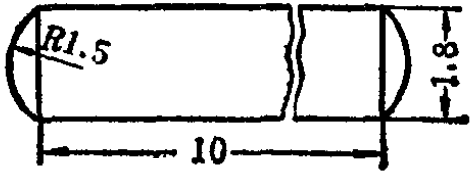
\includegraphics[width=5cm]{../pic/ltjh-ch2-xiti15-09.png}\\
    (第 9 题)
\end{minipage}

\end{enhancedline}
\end{xiaotis}

